\documentclass[USenglish,aspectratio=169]{beamer} % either 'ngerman' or 'USenglish'

\usetheme{metropolis}

% general
% \usepackage{babel}
% \usepackage{csquotes}
\usepackage{xcolor}
\usepackage{colortbl}
\usepackage{hyperref}
\usepackage[
  backend=biber,
  url=false,
  style=ieee,
  citestyle=ieee
]{biblatex}
\addbibresource{references.bib}

\usepackage{listings}
\usepackage{soul}
% tables
\usepackage{tabularx}
\usepackage{array}
\usepackage{multirow}
\usepackage{multicol}
\usepackage{booktabs}
\usepackage{makecell} % for line breaks in table cells

% math
\usepackage{amsmath}
\usepackage{amsfonts}
\usepackage{amssymb}
\usepackage{amsthm}
\usepackage{centernot}
\usepackage{bm}

% figures
\usepackage{graphicx}
\usepackage{tikz}
\usepackage{pgfplots}
\usepackage{listings}

% \usepackage{appendixnumberbeamer} % might cause arithmetic overflow error!
\usepackage{glossaries}
\usepackage{adjustbox}

\usepackage{listings}
\lstset{
    escapeinside={*@}{@*},
    showspaces=false,
    showstringspaces=false,
    showtabs=false
    xleftmargin=1pt,
    xrightmargin=1pt,
    aboveskip=1pt,
    belowskip=1pt,
    columns=fullflexible
}
\setlength\fboxsep{1pt}

\title{Extending Automerge: Undo and Redo}
% \subtitle{A Guided Research Project with Martin Kleppmann}
\author{Leo Stewen, Martin Kleppmann}
\date{October, 2023}

\graphicspath{{figures/}{../figures/}}
\hypersetup{
  pdftitle=\title,
  pdfauthor=\author,
  bookmarksopen=true,
  hidelinks,
}

\definecolor{opset1}{rgb}{0, 0.5, 1}
\definecolor{opset2}{rgb}{0.5, 0, 1}
\definecolor{opset3}{rgb}{0, 0.5, 0}
\definecolor{opset4}{rgb}{1, 0, 0}
\metroset{numbering=fraction,progressbar=frametitle,block=fill}
\setbeamertemplate{section in toc}[sections numbered]
\def\black{black}
\def\green{green!60!black}
\def\red{red}

\usetikzlibrary{
  quotes,
  automata,
  positioning,
  arrows,
  arrows.meta,
  calc,
  backgrounds,
  decorations.pathreplacing,
  calc,
  positioning, 
  fit
}

\tikzset{
  op/.style={
    font=\footnotesize,
    state,
    minimum size=50pt,
    fill=white,
  },
  inv/.style={
    font=\footnotesize,
    minimum size=50pt,
    circle,
    color=transparent,
  },
  head/.style={
    op,
    accepting,
  },
  edge/.style={
    ->,
    >={Stealth[round]},
  },
  pred/.style={
    edge,
  },
  anchorref/.style={
    edge,
    blue,
    dashed,
  },
  stepmarker/.style={
    font=\footnotesize,
    fill=black!10,
  },
  stepline/.style={
    edge,
    black!70,
    dotted,
    semithick,
    -,
  },
}
\newcommand{\op}[3][op]{$\mathit{#1}_{#2}^{#3}$} % with op kind
\newcommand{\opid}[2]{$\mathit{_{#1}^{#2}}$}
\newcommand{\setop}[4][set]{$\mathit{#1_{#2}^{\textbf{#3}}}{(#4)}$}
\newcommand{\putop}[4][put]{$\mathit{#1_{#2}^{\textbf{#3}}}{(#4)}$}
\newcommand{\delop}[3][del]{$\mathit{#1_{#2}^{\textbf{#3}}}{()}$}
\newcommand{\undop}[5][undo]{$\mathit{#1_{#2}^{\textbf{#3}}}{(_{#4}^{#5})}$}
\newcommand{\redop}[5][redo]{$\mathit{#1_{#2}^{\textbf{#3}}}{(_{#4}^{#5})}$}
\newcommand{\movop}[4][move]{$\mathit{#1_{#2}^{\textbf{#3}}}{(#4)}$}
\newcommand{\restop}[5][rest]{$\mathit{#1_{#2}^{\textbf{#3}}}{(_{#4}^{#5})}$}
\newcommand{\stack}[1]{$[$#1$]$}
\def\setabbr{s}
\def\restabbr{rs}
\newcommand{\setopkind}{\textit{SetOp}}
\newcommand{\restopkind}{\textit{RestoreOp}}
\newcommand{\terminalopkind}{\textit{TerminalOp}}
\newcommand{\opidtrace}{\textit{OpIdTrace}}

\begin{document}

\begin{frame}
\maketitle
\end{frame}

% \begin{frame}{Contents}
% \tableofcontents
% \end{frame}

\subsection{Semantics with Multiple Registers}

\begin{frame}[fragile]
  \begin{figure}
    \begin{adjustbox}{max totalsize={\textwidth}{0.75\textheight},center}
      \begin{tikzpicture}[node distance=0.23cm]
        \coordinate (c1) at (0,0);

        \tikzset{
          canvas/.style={
            rectangle,
            draw,
            anchor = west,
            inner sep = 4pt,
          },
          rect/.style={
            rectangle,
            minimum width = 1.2cm, 
            minimum height = 0.5cm,
            inner sep = 0.1cm,
            text = white,
            fill = #1,
          },
          optrans/.style={
            <-,bend right=90,>={Stealth[round]},
            swap,
            black!70,
          },
          casediv/.style={
            black!70,
          },
        }

        \def\black{black}
        \def\green{green!60!black}
        \def\red{red}
        \def\upperoffset{20pt}
        \def\loweroffset{50pt}

        \onslide<1->{
        \node[
          canvas,
          label={[]above:(1a)},
        ] (1a) at (c1) {
          \begin{tikzpicture}[node distance=3pt]
            \node[
                rect=\black,
              ] (r1) at (0,0) {\vphantom{bg}black};
            \node[
                rect=\black,
                below = of r1,
              ] (r2) {\vphantom{bg}black};
          \end{tikzpicture}
        };
        }

        \onslide<3->{
        \node[
          canvas,
          label={[]above:(1b)},
          right = of 1a,
        ] (1b) {
          \begin{tikzpicture}[node distance=3pt]
            \node[
                rect=\red,
              ] (r1) at (0,0) {\vphantom{bg}red};
            \node[
                rect=\black,
                below = of r1,
              ] (r2) {\vphantom{bg}black};
          \end{tikzpicture}
        } edge (1a);
        }

        \onslide<5->{
        \node[
          canvas,
          label={[]above:(1c)},
          right = of 1b,
        ] (1c) {
          \begin{tikzpicture}[node distance=3pt]
            \node[
                rect=\red,
              ] (r1) at (0,0) {\vphantom{bg}red};
            \node[
                rect=\green,
                below = of r1,
              ] (r2) {\vphantom{bg}green};
          \end{tikzpicture}
        } edge (1b);
        }

        \onslide<7->{
        \node[
          canvas,
          label={[]above:(1d)},
          right = of 1c,
        ] (1d) {
          \begin{tikzpicture}[node distance=3pt]
            \node[
                rect=\black,
              ] (r1) at (0,0) {\vphantom{bg}black};
            \node[
                rect=\green,
                below = of r1,
              ] (r2) {\vphantom{bg}green};
          \end{tikzpicture}
        } edge (1c);
        }

        \onslide<9->{
        \node[
          canvas,
          label={[]above:(1e)},
          right = of 1d,
        ] (1e) {
          \begin{tikzpicture}[node distance=3pt]
            \node[
                rect=\red,
              ] (r1) at (0,0) {\vphantom{bg}red};
            \node[
                rect=\green,
                below = of r1,
              ] (r2) {\vphantom{bg}green};
          \end{tikzpicture}
        } edge (1d);
        }

        \coordinate (d1s) at ($(1a.north)!0.5!(1b.north)+(0,+\upperoffset)$);
        \coordinate (d1e) at ($(1a.north)!0.5!(1b.north)+(0,-\loweroffset)$);

        \coordinate (d2s) at ($(1b.north)!0.5!(1c.north)+(0,+\upperoffset)$);
        \coordinate (d2e) at ($(1b.north)!0.5!(1c.north)+(0,-\loweroffset)$);

        \coordinate (d3s) at ($(1c.north)!0.5!(1d.north)+(0,+\upperoffset)$);
        \coordinate (d3e) at ($(1c.north)!0.5!(1d.north)+(0,-\loweroffset)$);

        \coordinate (d4s) at ($(1d.north)!0.5!(1e.north)+(0,+\upperoffset)$);
        \coordinate (d4e) at ($(1d.north)!0.5!(1e.north)+(0,-\loweroffset)$);

        \onslide<2->{
        \draw[stepline] (d1s) -- (d1e);
        \draw (1b.north)+(-0.2cm,+\upperoffset) edge ["A set",optrans] ($(1a.north)+(0,+\upperoffset)$);
        }

        \onslide<4->{
        \draw (1c.north)+(-0.2cm,+\upperoffset) edge ["B set",optrans] ($(1b.north)+(0,+\upperoffset)$);
        \draw[stepline] (d2s) -- (d2e);
        }

        \onslide<6->{
        \draw (1d.north)+(-0.2cm,+\upperoffset) edge ["A undo",optrans] ($(1c.north)+(0,+\upperoffset)$);
        \draw[stepline] (d3s) -- (d3e);
        }

        \onslide<8->{
        \draw (1e.north)+(-0.2cm,+\upperoffset) edge ["A redo",optrans] ($(1d.north)+(0,+\upperoffset)$);
        \draw[stepline] (d4s) -- (d4e);
        }

      \end{tikzpicture}
    \end{adjustbox}
    \caption{Canvas with two replicated registers.}\label{fig:intro-two-registers-front}
  \end{figure}
\end{frame}

\begin{frame}[fragile]
  \begin{figure}
    \begin{adjustbox}{max totalsize={\textwidth}{0.75\textheight},center}
      \begin{tikzpicture}[node distance=0.23cm]
        \coordinate (c1) at (0,0);

        \tikzset{
          canvas/.style={
            rectangle,
            draw,
            anchor = west,
            inner sep = 4pt,
          },
          rect/.style={
            rectangle,
            minimum width = 1.2cm, 
            minimum height = 0.5cm,
            inner sep = 0.1cm,
            text = white,
            fill = #1,
          },
          optrans/.style={
            <-,bend right=90,>={Stealth[round]},
            swap,
            black!70,
          },
          casediv/.style={
            black!70,
          },
        }

        \def\black{black}
        \def\green{green!60!black}
        \def\red{red}
        \def\upperoffset{20pt}
        \def\loweroffset{50pt}

        \coordinate (d1s) at ($(1a.north)!0.5!(1b.north)+(0,+\upperoffset)$);
        \coordinate (d1e) at ($(1a.north)!0.5!(1b.north)+(0,-\loweroffset)$);

        \coordinate (d2s) at ($(1b.north)!0.5!(1c.north)+(0,+\upperoffset)$);
        \coordinate (d2e) at ($(1b.north)!0.5!(1c.north)+(0,-\loweroffset)$);

        \coordinate (d3s) at ($(1c.north)!0.5!(1d.north)+(0,+\upperoffset)$);
        \coordinate (d3e) at ($(1c.north)!0.5!(1d.north)+(0,-\loweroffset)$);

        \coordinate (d4s) at ($(1d.north)!0.5!(1e.north)+(0,+\upperoffset)$);
        \coordinate (d4e) at ($(1d.north)!0.5!(1e.north)+(0,-\loweroffset)$);

        \onslide<2->{
        \draw (1b.north)+(-0.2cm,+\upperoffset) edge ["A set",optrans] ($(1a.north)+(0,+\upperoffset)$);
        \draw[stepline] (d1s) -- (d1e);
        }

        \onslide<4->{
        \draw (1c.north)+(-0.2cm,+\upperoffset) edge ["B set",optrans] ($(1b.north)+(0,+\upperoffset)$);
        \draw[stepline] (d2s) -- (d2e);
        }

        \onslide<6->{
        \draw (1d.north)+(-0.2cm,+\upperoffset) edge ["A undo",optrans] ($(1c.north)+(0,+\upperoffset)$);
        \draw[stepline] (d3s) -- (d3e);
        }

        \onslide<8->{
        \draw (1e.north)+(-0.2cm,+\upperoffset) edge ["A redo",optrans] ($(1d.north)+(0,+\upperoffset)$);
        \draw[stepline] (d4s) -- (d4e);
        }

        %%%%
        
        \onslide<1->{
        \node[
          canvas,
          label={[]above:(2a)},
        ] (2a) at (c1) {
          \begin{tikzpicture}[node distance=3pt]
            \node[
                rect=\black,
              ] (r1) at (0,0) {\vphantom{bg}black};
          \end{tikzpicture}
        };
        }

        \onslide<3->{
        \node[
          canvas,
          label={[]above:(2b)},
          right = of 2a,
        ] (2b) {
          \begin{tikzpicture}[node distance=3pt]
            \node[
                rect=\red,
              ] (r1) at (0,0) {\vphantom{bg}red};
          \end{tikzpicture}
        } edge (2a);
        }

        \onslide<5->{
        \node[
          canvas,
          label={[]above:(2c)},
          right = of 2b,
        ] (2c) {
          \begin{tikzpicture}[node distance=3pt]
            \node[
                rect=\green,
              ] (r1) at (0,0) {\vphantom{bg}green};
          \end{tikzpicture}
        } edge (2b);
        }

        %%%

        \onslide<7->{
        \node[
          canvas,
          label={[]above:(2d1)},
          right = of 2c,
        ] (2d1) {
          \begin{tikzpicture}[node distance=3pt]
            \node[
                rect=\black,
              ] (r1) at (0,0) {\vphantom{bg}black};
          \end{tikzpicture}
        } edge (2c);
        }

        \onslide<9->{
        \node[
          canvas,
          label={[]above:(2e2)},
          right = of 2d1,
        ] (2d1e2) {
          \begin{tikzpicture}[node distance=3pt]
            \node[
                rect=\green,
              ] (r1) at (0,0) {\vphantom{bg}green};
          \end{tikzpicture}
        } edge (2d1);
        }

        \only<10->{
        \node [fill=white,anchor=center,draw,rounded corners] at (4.2,-2.0) {
            \includegraphics[height=30px]{figures/gsheets.png}
            \includegraphics[height=30px]{figures/gslides.png}
            \includegraphics[height=30px]{figures/figma.png}
            \includegraphics[height=30px]{figures/powerpoint.png}
            \includegraphics[height=30px]{figures/excel.png}
            \only<10>{
              \includegraphics[height=30px]{figures/miro.png}%
            }
            \only<11>{
              \includegraphics[height=30px]{figures/miro_crossed_out.png}%
            }
        };
        }

      \end{tikzpicture}
    \end{adjustbox}
    \caption{Canvas with one replicated register.}\label{fig:intro-one-register-back}
  \end{figure}
\end{frame}

\subsection{Background}

\begin{frame}[fragile]{Why Replicated Registers, if Automerge is a JSON CRDT?}
  \begin{figure}
    \center
    \includegraphics[height=0.5\textheight]{paper.png}
  \end{figure}
  \pause

  \begin{figure}
  \begin{adjustbox}{max totalsize={\textwidth}{0.75\textheight},center}
  \begin{tikzpicture}[node distance=60pt]
     \node[] (json) at (0,0) {
        \begin{lstlisting}
        {
          *@\colorbox{opset1!10}{A: a,}@*
          *@\colorbox{opset2!10}{B: [b1, b2]}@*
        }
        \end{lstlisting}};

      \pause
      \node[right=90pt of json,rectangle,draw] (box) {
          Replicated Registers
        };

      \draw[-latex,->] (box.west) to [bend right=45] (1.3,0.4);

      \draw[-latex,->] (box.west) to [bend left=55] (1.0,-0.6);
      \draw[-latex,->] (box.west) to [bend left=50] (1.6,-0.6);
      \draw[-latex,->] (box.west) to [bend left=45] (2.3,-0.6);
  \end{tikzpicture}
  \end{adjustbox}
  \end{figure}
\end{frame}

\subsection{Edge Cases}

% Undo has to restore conflicts if it undoes a merge operation.
\setbeamercovered{transparent=35}
\begin{frame}[fragile]{Edge Cases to Consider (1)}
  \begin{figure}
    \begin{adjustbox}{max totalsize={\textwidth}{0.75\textheight},center}
\begin{tikzpicture}[node distance=60pt]
  \tikzset{
    register/.style={
      anchor=west,
      xshift=-90pt,
    },
  }
  \def\dist{18pt}

  \only<1>{
    \node[register] (vals) at (0, 2) {\textbf{Register: }\stack{
          \colorbox{black}{\phantom{R}}
    }};
  }
  \only<2,4>{
    \node[register] (vals) at (0, 2) {\textbf{Register: }\stack{
          \colorbox{green}{\phantom{R}}, \colorbox{red}{\phantom{R}}
    }};
  }
  \only<3>{
    \node[register] (vals) at (0, 2) {\textbf{Register: }\stack{
          \colorbox{blue}{\phantom{R}}
    }};
  }

  % nodes and edges
  \visible<1->{
    \node[op] (a1) at (0, 0) {\setop{1}{A}{\colorbox{black}{\phantom{R}}}};
  }

  \visible<2->{
    \node[op,above right=\dist of a1] (a2) {\setop{2}{A}{\colorbox{red}{\phantom{R}}}} edge [pred] (a1);
    \node[op,below right=\dist of a1] (b2) {\setop{2}{B}{\colorbox{green}{\phantom{R}}}} edge [pred] (a1);
  }

  \visible<3->{
    \node[op,below right=\dist of a2] (a3) {\setop{3}{A}{\colorbox{blue}{\phantom{R}}}} edge [pred] (a2) edge [pred] (b2);
  }

  \visible<4->{
    \node[op,above right=\dist of a3] (a4) {\undop{4}{A}{3}{A}} edge [pred] (a3) edge [anchorref,bend right=30] (a3);
  }

  % invisible
  \node[inv,below right=\dist of a4] (b5) {\phantom{\redop{5}{B}{4}{B}}};
\end{tikzpicture}
\end{adjustbox}
\caption{
  Undo of a merge op.
}\label{fig:undo-merge-op}
\end{figure}
\end{frame}
\setbeamercovered{invisible}

\setbeamercovered{transparent=35}
\begin{frame}[fragile]{Edge Cases to Consider (2)}
  \begin{figure}
    \begin{adjustbox}{max totalsize={\textwidth}{0.75\textheight},center}
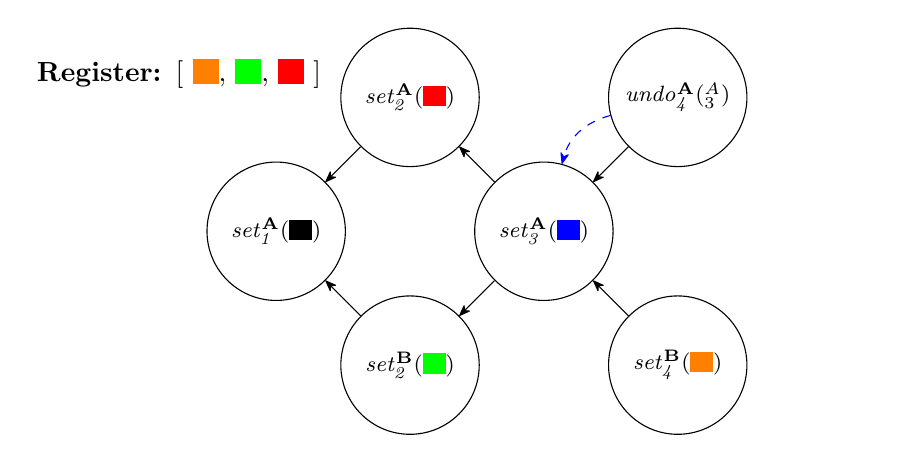
\begin{tikzpicture}[node distance=60pt]
  \tikzset{
    register/.style={
      anchor=west,
      xshift=-90pt,
    },
  }
  \def\dist{18pt}

  \only<1->{
    \node[register] (vals) at (0, 2) {\textbf{Register: }\stack{
          \colorbox{orange}{\phantom{R}}, \colorbox{green}{\phantom{R}}, \colorbox{red}{\phantom{R}}
    }};
  }

  % nodes and edges
  \node[op] (a1) at (0, 0) {\setop{1}{A}{\colorbox{black}{\phantom{R}}}};

  \node[op,above right=\dist of a1] (a2) {\setop{2}{A}{\colorbox{red}{\phantom{R}}}} edge [pred] (a1);
  \node[op,below right=\dist of a1] (b2) {\setop{2}{B}{\colorbox{green}{\phantom{R}}}} edge [pred] (a1);

  \node[op,below right=\dist of a2] (a3) {\setop{3}{A}{\colorbox{blue}{\phantom{R}}}} edge [pred] (a2) edge [pred] (b2);

  \node[op,above right=\dist of a3] (a4) {\undop{4}{A}{3}{A}} edge [pred] (a3) edge [anchorref,bend right=30] (a3);

  \node[op,below right=\dist of a3] (b4) {\setop{4}{B}{\colorbox{orange}{\phantom{R}}}} edge [pred] (a3);

  % invisible
  \node[inv,below right=\dist of a4] (b5) {\phantom{\redop{5}{B}{4}{B}}};
\end{tikzpicture}
\end{adjustbox}
\caption{
  Concurrent undo and set op.
}\label{fig:concurrent-undo-set}
\end{figure}
\end{frame}
\setbeamercovered{invisible}

\setbeamercovered{transparent=35}
\begin{frame}[fragile]{Edge Cases to Consider (3)}
  \begin{figure}
    \begin{adjustbox}{max totalsize={\textwidth}{0.75\textheight},center}
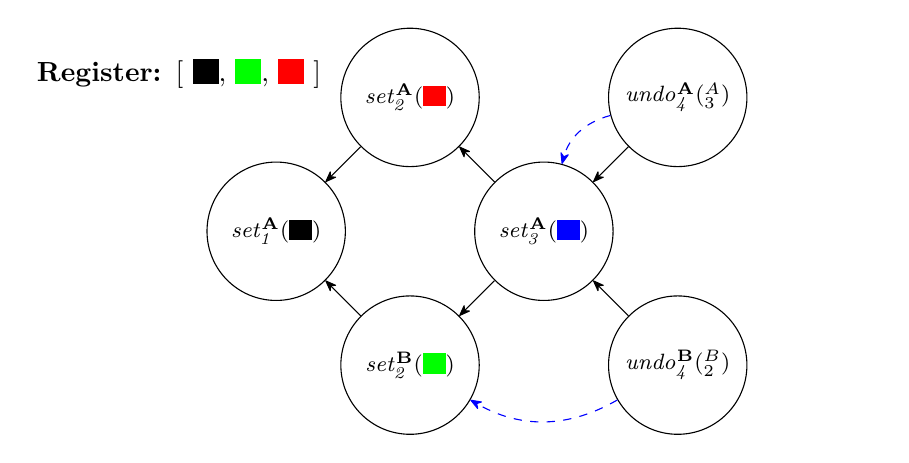
\begin{tikzpicture}[node distance=60pt]
  \tikzset{
    register/.style={
      anchor=west,
      xshift=-90pt,
    },
  }
  \def\dist{18pt}

  \only<1->{
    \node[register] (vals) at (0, 2) {\textbf{Register: }\stack{
          \colorbox{black}{\phantom{R}}, \colorbox{green}{\phantom{R}}, \colorbox{red}{\phantom{R}}
    }};
  }

  % nodes and edges
  \node[op] (a1) at (0, 0) {\setop{1}{A}{\colorbox{black}{\phantom{R}}}};

  \node[op,above right=\dist of a1] (a2) {\setop{2}{A}{\colorbox{red}{\phantom{R}}}} edge [pred] (a1);
  \node[op,below right=\dist of a1] (b2) {\setop{2}{B}{\colorbox{green}{\phantom{R}}}} edge [pred] (a1);

  \node[op,below right=\dist of a2] (a3) {\setop{3}{A}{\colorbox{blue}{\phantom{R}}}} edge [pred] (a2) edge [pred] (b2);

  \node[op,above right=\dist of a3] (a4) {\undop{4}{A}{3}{A}} edge [pred] (a3) edge [anchorref,bend right=30] (a3);

  \node[op,below right=\dist of a3] (b4) {\undop{4}{B}{2}{B}} edge [pred] (a3) edge [anchorref,bend left=30] (b2);

  % invisible
  \node[inv,below right=\dist of a4] (b5) {\phantom{\redop{5}{B}{4}{B}}};
\end{tikzpicture}
\end{adjustbox}
\caption{
  Concurrent undo ops.
}\label{fig:concurrent-undos}
\end{figure}
\end{frame}
\setbeamercovered{invisible}

\setbeamercovered{transparent=35}
\begin{frame}[fragile]{Edge Cases to Consider (4)}
  \begin{figure}
    \begin{adjustbox}{max totalsize={\textwidth}{0.75\textheight},center}
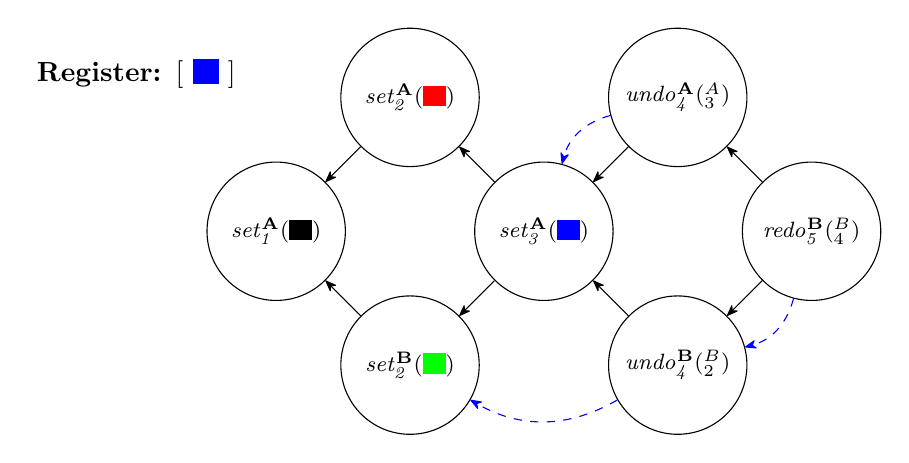
\begin{tikzpicture}[node distance=60pt]
  \tikzset{
    register/.style={
      anchor=west,
      xshift=-90pt,
    },
  }
  \def\dist{18pt}

  \only<1->{
    \node[register] (vals) at (0, 2) {\textbf{Register: }\stack{
          \colorbox{blue}{\phantom{R}}
    }};
  }

  % nodes and edges
  \node[op] (a1) at (0, 0) {\setop{1}{A}{\colorbox{black}{\phantom{R}}}};

  \node[op,above right=\dist of a1] (a2) {\setop{2}{A}{\colorbox{red}{\phantom{R}}}} edge [pred] (a1);
  \node[op,below right=\dist of a1] (b2) {\setop{2}{B}{\colorbox{green}{\phantom{R}}}} edge [pred] (a1);

  \node[op,below right=\dist of a2] (a3) {\setop{3}{A}{\colorbox{blue}{\phantom{R}}}} edge [pred] (a2) edge [pred] (b2);

  \node[op,above right=\dist of a3] (a4) {\undop{4}{A}{3}{A}} edge [pred] (a3) edge [anchorref,bend right=30] (a3);

  \node[op,below right=\dist of a3] (b4) {\undop{4}{B}{2}{B}} edge [pred] (a3) edge [anchorref,bend left=30] (b2);

  \node[op,below right=\dist of a4] (b5) {\redop{5}{B}{4}{B}} edge [pred] (b4) edge [pred] (a4) edge [anchorref,bend left=30] (b4);
\end{tikzpicture}
\end{adjustbox}
\caption{
  Redo restores state prior to its corresponding undo.
}\label{fig:edge-case-3}
\end{figure}
\end{frame}
\setbeamercovered{invisible}

\subsection{Evaluation}

\begin{frame}{Constant Runtime for Common Editing Scenarios}
  \begin{figure}
  \begin{adjustbox}{max totalsize={\textwidth}{0.75\textheight},center}
  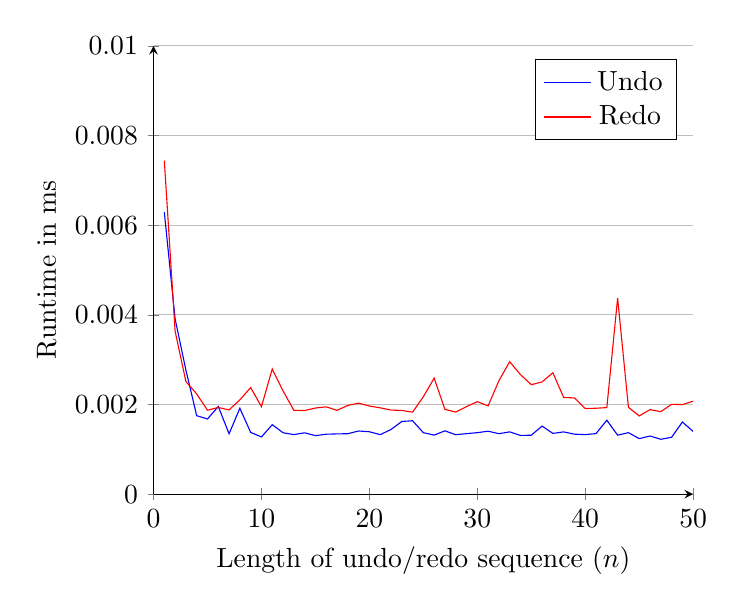
\begin{tikzpicture}
  \begin{axis}[
    xlabel={Length of undo/redo sequence ($n$)},
    ylabel={Runtime in ms},
    xmin=0,
    axis x line=bottom,
    axis y line=left,
    ymin=0,
    ymax=0.010,
    legend pos=north east,
    ymajorgrids=true,
    yticklabel style={
      /pgf/number format/fixed,
      /pgf/number format/precision=5
    },
    scaled y ticks=false 
  ]

  % undo data
  \addplot[
    color=blue,
  ] coordinates {
  (1, 0.006290340563282371)
  (2, 0.003907741687726229)
  (3, 0.002766803983831778)
  (4, 0.0017496687069069594)
  (5, 0.0016760083672124892)
  (6, 0.001955396990524605)
  (7, 0.001345782628050074)
  (8, 0.0019154881010763347)
  (9, 0.0013770495424978435)
  (10, 0.001276014547329396)
  (11, 0.0015485882759094238)
  (12, 0.0013692353677470237)
  (13, 0.0013271856296341866)
  (14, 0.0013679209514521062)
  (15, 0.001304528908804059)
  (16, 0.0013366359926294535)
  (17, 0.0013435808941721916)
  (18, 0.00134780234657228)
  (19, 0.0014081033586990088)
  (20, 0.0013913525617681444)
  (21, 0.0013268127804622054)
  (22, 0.001440957625163719)
  (23, 0.0016200695536099374)
  (24, 0.0016375818522647023)
  (25, 0.0013710299390368164)
  (26, 0.0013164350239094347)
  (27, 0.0014119130210019648)
  (28, 0.0013253243814688176)
  (29, 0.0013492428988683969)
  (30, 0.0013712448126170784)
  (31, 0.0014037845248822123)
  (32, 0.0013481056957971305)
  (33, 0.0013890777481719851)
  (34, 0.0013086109538562596)
  (35, 0.001314542896579951)
  (36, 0.0015176087035797536)
  (37, 0.0013542969536501914)
  (38, 0.0013883131032343954)
  (39, 0.0013373843976296484)
  (40, 0.0013278163387440145)
  (41, 0.0013506945979315788)
  (42, 0.0016484785883221775)
  (43, 0.0013150325394235551)
  (44, 0.0013713290682062507)
  (45, 0.0012379433319438249)
  (46, 0.0012963268964085728)
  (47, 0.0012237174669280648)
  (48, 0.0012681810767389834)
  (49, 0.001609297381946817)
  (50, 0.0013969987630844116)
  };

  % redo data
  \addplot[
    color=red,
  ] coordinates {
  (1, 0.007437939144438133)
  (2, 0.003633987420471385)
  (3, 0.002511455590138212)
  (4, 0.0022350119543261826)
  (5, 0.0018720132065936923)
  (6, 0.0019328816561028361)
  (7, 0.00187860953155905)
  (8, 0.002103224309394136)
  (9, 0.0023768509563524276)
  (10, 0.001951182057382539)
  (11, 0.0027914689562749118)
  (12, 0.002302225591847673)
  (13, 0.0018702853412833065)
  (14, 0.001864643389126286)
  (15, 0.0019206689321435988)
  (16, 0.0019472866551950574)
  (17, 0.0018687470292206854)
  (18, 0.0019792676030192524)
  (19, 0.002029231225606054)
  (20, 0.001964766182936728)
  (21, 0.0019252107886131853)
  (22, 0.0018749097071122378)
  (23, 0.001866210310254246)
  (24, 0.0018289572326466441)
  (25, 0.0021713866444770247)
  (26, 0.002587106981081888)
  (27, 0.0018908421625383198)
  (28, 0.0018309024162590504)
  (29, 0.0019520004279911518)
  (30, 0.002062761748675257)
  (31, 0.001968364085769281)
  (32, 0.002528973447624594)
  (33, 0.002954049239633605)
  (34, 0.0026645801845006645)
  (35, 0.002441259188344702)
  (36, 0.002502664952771738)
  (37, 0.002708020620048046)
  (38, 0.002156659436877817)
  (39, 0.0021457494294736534)
  (40, 0.0019089243141934276)
  (41, 0.0019161189266014844)
  (42, 0.0019302570726722479)
  (43, 0.004374536831164733)
  (44, 0.0019373227842152119)
  (45, 0.0017444676195736974)
  (46, 0.0018851725617423654)
  (47, 0.001839210162870586)
  (48, 0.0020025315461680293)
  (49, 0.0019971978035755455)
  (50, 0.002073564799502492)
  };

  \legend{Undo, Redo}

  \end{axis}
  \end{tikzpicture}
  \end{adjustbox}
  \caption{
    Runtime of the last undo/redo operation in a sequence
    of $n$ consecutive undo/redo operations.
  }\label{fig:runtime-cons-undo-redo}
  \end{figure}
\end{frame}

\begin{frame}[standout]
  Questions? Feedback? \\
  \vspace{1.2em}
  \small
  \texttt{
    Reach us at \\
    \href{mailto:lstwn@mailbox.org}{lstwn@mailbox.org} \\
    \href{mailto:liangrun.da@tum.de}{liangrun.da@tum.de} \\
    \href{mailto:martin@kleppmann.com}{martin@kleppmann.com}
  } \\
  % TODO: upload paper
  LINK TO PAPERS! (as QR code?)
\end{frame}
\setbeamercovered{invisible}

\appendix{}

\begin{frame}[allowframebreaks]
    \printbibliography{}
\end{frame}

\section*{Backup Slides}

\subsection{Extended Semantics}

\begin{frame}[fragile]
  \begin{figure}
    \begin{adjustbox}{max totalsize={\textwidth}{0.75\textheight},center}
      \begin{tikzpicture}[node distance=0.23cm]
        \coordinate (c1) at (0,0);

        \tikzset{
          canvas/.style={
            rectangle,
            draw,
            anchor = west,
            inner sep = 4pt,
          },
          rect/.style={
            rectangle,
            minimum width = 1.2cm, 
            minimum height = 0.5cm,
            inner sep = 0.1cm,
            text = white,
            fill = #1,
          },
          optrans/.style={
            <-,bend right=90,>={Stealth[round]},
            swap,
            black!70,
          },
          casediv/.style={
            black!70,
          },
        }

        \def\black{black}
        \def\green{green!60!black}
        \def\red{red}
        \def\upperoffset{20pt}
        \def\loweroffset{50pt}

        \onslide<1->{
        \node[
          canvas,
          label={[]above:(1a)},
        ] (1a) at (c1) {
          \begin{tikzpicture}[node distance=3pt]
            \node[
                rect=\black,
              ] (r1) at (0,0) {\vphantom{bg}black};
            \node[
                rect=\black,
                below = of r1,
              ] (r2) {\vphantom{bg}black};
          \end{tikzpicture}
        };
        }

        \onslide<3->{
        \node[
          canvas,
          label={[]above:(1b)},
          right = of 1a,
        ] (1b) {
          \begin{tikzpicture}[node distance=3pt]
            \node[
                rect=\red,
              ] (r1) at (0,0) {\vphantom{bg}red};
            \node[
                rect=\black,
                below = of r1,
              ] (r2) {\vphantom{bg}black};
          \end{tikzpicture}
        } edge (1a);
        }

        \onslide<5->{
        \node[
          canvas,
          label={[]above:(1c)},
          right = of 1b,
        ] (1c) {
          \begin{tikzpicture}[node distance=3pt]
            \node[
                rect=\red,
              ] (r1) at (0,0) {\vphantom{bg}red};
            \node[
                rect=\green,
                below = of r1,
              ] (r2) {\vphantom{bg}green};
          \end{tikzpicture}
        } edge (1b);
        }

        \onslide<7->{
        \node[
          canvas,
          label={[]above:(1d)},
          right = of 1c,
        ] (1d) {
          \begin{tikzpicture}[node distance=3pt]
            \node[
                rect=\black,
              ] (r1) at (0,0) {\vphantom{bg}black};
            \node[
                rect=\green,
                below = of r1,
              ] (r2) {\vphantom{bg}green};
          \end{tikzpicture}
        } edge (1c);
        }

        \onslide<9->{
        \node[
          canvas,
          label={[]above:(1e)},
          right = of 1d,
        ] (1e) {
          \begin{tikzpicture}[node distance=3pt]
            \node[
                rect=\red,
              ] (r1) at (0,0) {\vphantom{bg}red};
            \node[
                rect=\green,
                below = of r1,
              ] (r2) {\vphantom{bg}green};
          \end{tikzpicture}
        } edge (1d);
        }

        \coordinate (d1s) at ($(1a.north)!0.5!(1b.north)+(0,+\upperoffset)$);
        \coordinate (d1e) at ($(1a.north)!0.5!(1b.north)+(0,-\loweroffset)$);

        \coordinate (d2s) at ($(1b.north)!0.5!(1c.north)+(0,+\upperoffset)$);
        \coordinate (d2e) at ($(1b.north)!0.5!(1c.north)+(0,-\loweroffset)$);

        \coordinate (d3s) at ($(1c.north)!0.5!(1d.north)+(0,+\upperoffset)$);
        \coordinate (d3e) at ($(1c.north)!0.5!(1d.north)+(0,-\loweroffset)$);

        \coordinate (d4s) at ($(1d.north)!0.5!(1e.north)+(0,+\upperoffset)$);
        \coordinate (d4e) at ($(1d.north)!0.5!(1e.north)+(0,-\loweroffset)$);

        \onslide<2->{
        \draw[stepline] (d1s) -- (d1e);
        \draw (1b.north)+(-0.2cm,+\upperoffset) edge ["A set",optrans] ($(1a.north)+(0,+\upperoffset)$);
        }

        \onslide<4->{
        \draw (1c.north)+(-0.2cm,+\upperoffset) edge ["B set",optrans] ($(1b.north)+(0,+\upperoffset)$);
        \draw[stepline] (d2s) -- (d2e);
        }

        \onslide<6->{
        \draw (1d.north)+(-0.2cm,+\upperoffset) edge ["A undo",optrans] ($(1c.north)+(0,+\upperoffset)$);
        \draw[stepline] (d3s) -- (d3e);
        }

        \onslide<8->{
        \draw (1e.north)+(-0.2cm,+\upperoffset) edge ["A redo",optrans] ($(1d.north)+(0,+\upperoffset)$);
        \draw[stepline] (d4s) -- (d4e);
        }

      \end{tikzpicture}
    \end{adjustbox}
    \caption{Canvas with two replicated registers.}\label{fig:intro-two-registers}
  \end{figure}
\end{frame}

\begin{frame}[fragile]
  \begin{figure}
    \begin{adjustbox}{max totalsize={\textwidth}{0.75\textheight},center}
      \begin{tikzpicture}[node distance=0.23cm]
        \coordinate (c1) at (0,-1.6);

        \tikzset{
          canvas/.style={
            rectangle,
            draw,
            anchor = west,
            inner sep = 4pt,
          },
          rect/.style={
            rectangle,
            minimum width = 1.2cm, 
            minimum height = 0.5cm,
            inner sep = 0.1cm,
            text = white,
            fill = #1,
          },
          optrans/.style={
            <-,bend right=90,>={Stealth[round]},
            swap,
            black!70,
          },
          casediv/.style={
            black!70,
          },
        }

        \def\black{black}
        \def\green{green!60!black}
        \def\red{red}
        \def\upperoffset{20pt}
        \def\loweroffset{120pt}

        \coordinate (d1s) at ($(1a.north)!0.5!(1b.north)+(0,+\upperoffset)$);
        \coordinate (d1e) at ($(1a.north)!0.5!(1b.north)+(0,-\loweroffset)$);

        \coordinate (d2s) at ($(1b.north)!0.5!(1c.north)+(0,+\upperoffset)$);
        \coordinate (d2e) at ($(1b.north)!0.5!(1c.north)+(0,-\loweroffset)$);

        \coordinate (d3s) at ($(1c.north)!0.5!(1d.north)+(0,+\upperoffset)$);
        \coordinate (d3e) at ($(1c.north)!0.5!(1d.north)+(0,-\loweroffset)$);

        \coordinate (d4s) at ($(1d.north)!0.5!(1e.north)+(0,+\upperoffset)$);
        \coordinate (d4e) at ($(1d.north)!0.5!(1e.north)+(0,-\loweroffset)$);

        \onslide<2->{
        \draw (1b.north)+(-0.2cm,+\upperoffset) edge ["A set",optrans] ($(1a.north)+(0,+\upperoffset)$);
        \draw[stepline] (d1s) -- (d1e);
        }

        \onslide<4->{
        \draw (1c.north)+(-0.2cm,+\upperoffset) edge ["B set",optrans] ($(1b.north)+(0,+\upperoffset)$);
        \draw[stepline] (d2s) -- (d2e);
        }

        \onslide<6->{
        \draw (1d.north)+(-0.2cm,+\upperoffset) edge ["A undo",optrans] ($(1c.north)+(0,+\upperoffset)$);
        \draw[stepline] (d3s) -- (d3e);
        }

        \onslide<9->{
        \draw (1e.north)+(-0.2cm,+\upperoffset) edge ["A redo",optrans] ($(1d.north)+(0,+\upperoffset)$);
        \draw[stepline] (d4s) -- (d4e);
        }

        %%%%
        
        \onslide<1->{
        \node[
          canvas,
          label={[]above:(2a)},
        ] (2a) at (c1) {
          \begin{tikzpicture}[node distance=3pt]
            \node[
                rect=\black,
              ] (r1) at (0,0) {\vphantom{bg}black};
          \end{tikzpicture}
        };
        }

        \onslide<3->{
        \node[
          canvas,
          label={[]above:(2b)},
          right = of 2a,
        ] (2b) {
          \begin{tikzpicture}[node distance=3pt]
            \node[
                rect=\red,
              ] (r1) at (0,0) {\vphantom{bg}red};
          \end{tikzpicture}
        } edge (2a);
        }

        \onslide<5->{
        \node[
          canvas,
          label={[]above:(2c)},
          right = of 2b,
        ] (2c) {
          \begin{tikzpicture}[node distance=3pt]
            \node[
                rect=\green,
              ] (r1) at (0,0) {\vphantom{bg}green};
          \end{tikzpicture}
        } edge (2b);
        }

        %%%

        \onslide<8->{
        \node[
          canvas,
          label={[]above:(2d1)},
          above right = of 2c,
          xshift=+2pt,
          yshift=+4pt,
        ] (2d1) {
          \begin{tikzpicture}[node distance=3pt]
            \node[
                rect=\black,
              ] (r1) at (0,0) {\vphantom{bg}black};
          \end{tikzpicture}
        } edge (2c);
        }

        \onslide<11->{
        \node[
          canvas,
          label={[]above:(2e1)},
          above right = of 2d1,
          xshift=+2pt,
          yshift=-7pt,
        ] (2d1e1) {
          \begin{tikzpicture}[node distance=3pt]
            \node[
                rect=\red,
              ] (r1) at (0,0) {\vphantom{bg}red};
          \end{tikzpicture}
        } edge (2d1);
        }

        \onslide<11->{
        \node[
          canvas,
          label={[]above:(2e2)},
          below right = of 2d1,
          xshift=+2pt,
          yshift=+7pt,
        ] (2d1e2) {
          \begin{tikzpicture}[node distance=3pt]
            \node[
                rect=\green,
              ] (r1) at (0,0) {\vphantom{bg}green};
          \end{tikzpicture}
        } edge (2d1);
        }

        %%%

        \onslide<7->{
        \node[
          canvas,
          label={[]above:(2d2)},
          below right = of 2c,
          xshift=+2pt,
          yshift=-4pt,
        ] (2d2) {
          \begin{tikzpicture}[node distance=3pt]
            \node[
                rect=\red,
              ] (r1) at (0,0) {\vphantom{bg}red};
          \end{tikzpicture}
        } edge (2c);
        }

        \onslide<10->{
        \node[
          canvas,
          label={[]above:(2e3)},
          right = of 2d2,
        ] (2e2) {
          \begin{tikzpicture}[node distance=3pt]
            \node[
                rect=\green,
              ] (r1) at (0,0) {\vphantom{bg}green};
          \end{tikzpicture}
        } edge (2d2);
        }

      \end{tikzpicture}
    \end{adjustbox}
    \caption{Canvas with one replicated register.}\label{fig:intro-one-register}
  \end{figure}
\end{frame}

\setbeamercovered{transparent}
\begin{frame}[fragile]
  \begin{figure}
    \begin{adjustbox}{max totalsize={\textwidth}{0.75\textheight},center}
      \begin{tikzpicture}[node distance=0.23cm]
        \coordinate (c1) at (0,-1.6);

        \tikzset{
          canvas/.style={
            rectangle,
            draw,
            anchor = west,
            inner sep = 4pt,
          },
          rect/.style={
            rectangle,
            minimum width = 1.2cm, 
            minimum height = 0.5cm,
            inner sep = 0.1cm,
            text = white,
            fill = #1,
          },
          optrans/.style={
            <-,bend right=90,>={Stealth[round]},
            swap,
            black!70,
          },
          casediv/.style={
            black!70,
          },
        }

        \def\black{black}
        \def\green{green!60!black}
        \def\red{red}
        \def\upperoffset{20pt}
        \def\loweroffset{120pt}

        \coordinate (d1s) at ($(1a.north)!0.5!(1b.north)+(0,+\upperoffset)$);
        \coordinate (d1e) at ($(1a.north)!0.5!(1b.north)+(0,-\loweroffset)$);

        \coordinate (d2s) at ($(1b.north)!0.5!(1c.north)+(0,+\upperoffset)$);
        \coordinate (d2e) at ($(1b.north)!0.5!(1c.north)+(0,-\loweroffset)$);

        \coordinate (d3s) at ($(1c.north)!0.5!(1d.north)+(0,+\upperoffset)$);
        \coordinate (d3e) at ($(1c.north)!0.5!(1d.north)+(0,-\loweroffset)$);

        \coordinate (d4s) at ($(1d.north)!0.5!(1e.north)+(0,+\upperoffset)$);
        \coordinate (d4e) at ($(1d.north)!0.5!(1e.north)+(0,-\loweroffset)$);

        \draw (1b.north)+(-0.2cm,+\upperoffset) edge ["A set",optrans] ($(1a.north)+(0,+\upperoffset)$);
        \draw[stepline] (d1s) -- (d1e);

        \draw (1c.north)+(-0.2cm,+\upperoffset) edge ["B set",optrans] ($(1b.north)+(0,+\upperoffset)$);
        \draw[stepline] (d2s) -- (d2e);

        \draw (1d.north)+(-0.2cm,+\upperoffset) edge ["A undo",optrans] ($(1c.north)+(0,+\upperoffset)$);
        \draw[stepline] (d3s) -- (d3e);

        \draw (1e.north)+(-0.2cm,+\upperoffset) edge ["A redo",optrans] ($(1d.north)+(0,+\upperoffset)$);
        \draw[stepline] (d4s) -- (d4e);

        %%%%
        
        \onslide<1-2>{
        \node[
          canvas,
          label={[]above:(2a)},
        ] (2a) at (c1) {
          \begin{tikzpicture}[node distance=3pt]
            \node[
                rect=\black,
              ] (r1) at (0,0) {\vphantom{bg}black};
          \end{tikzpicture}
        };

        \node[
          canvas,
          label={[]above:(2b)},
          right = of 2a,
        ] (2b) {
          \begin{tikzpicture}[node distance=3pt]
            \node[
                rect=\red,
              ] (r1) at (0,0) {\vphantom{bg}red};
          \end{tikzpicture}
        } edge (2a);

        \node[
          canvas,
          label={[]above:(2c)},
          right = of 2b,
        ] (2c) {
          \begin{tikzpicture}[node distance=3pt]
            \node[
                rect=\green,
              ] (r1) at (0,0) {\vphantom{bg}green};
          \end{tikzpicture}
        } edge (2b);

        %%%

        \node[
          canvas,
          label={[]above:(2d1)},
          above right = of 2c,
          xshift=+2pt,
          yshift=+4pt,
        ] (2d1) {
          \begin{tikzpicture}[node distance=3pt]
            \node[
                rect=\black,
              ] (r1) at (0,0) {\vphantom{bg}black};
          \end{tikzpicture}
        } edge (2c);
        }

        \onslide<1>{
        \node[
          canvas,
          label={[]above:(2e1)},
          above right = of 2d1,
          xshift=+2pt,
          yshift=-7pt,
        ] (2d1e1) {
          \begin{tikzpicture}[node distance=3pt]
            \node[
                rect=\red,
              ] (r1) at (0,0) {\vphantom{bg}red};
          \end{tikzpicture}
        } edge (2d1);
        }

        \onslide<1-2>{
        \node[
          canvas,
          label={[]above:(2e2)},
          below right = of 2d1,
          xshift=+2pt,
          yshift=+7pt,
        ] (2d1e2) {
          \begin{tikzpicture}[node distance=3pt]
            \node[
                rect=\green,
              ] (r1) at (0,0) {\vphantom{bg}green};
          \end{tikzpicture}
        } edge (2d1);
        }

        %%%

        \onslide<1>{
        \node[
          canvas,
          label={[]above:(2d2)},
          below right = of 2c,
          xshift=+2pt,
          yshift=-4pt,
        ] (2d2) {
          \begin{tikzpicture}[node distance=3pt]
            \node[
                rect=\red,
              ] (r1) at (0,0) {\vphantom{bg}red};
          \end{tikzpicture}
        } edge (2c);

        \node[
          canvas,
          label={[]above:(2e3)},
          right = of 2d2,
        ] (2e2) {
          \begin{tikzpicture}[node distance=3pt]
            \node[
                rect=\green,
              ] (r1) at (0,0) {\vphantom{bg}green};
          \end{tikzpicture}
        } edge (2d2);
        }

      \end{tikzpicture}
    \end{adjustbox}
    \caption{Canvas with one replicated register.}\label{fig:intro-one-register-chosen-path}
  \end{figure}
\end{frame}

\subsection{Global vs Local Undo}

\setbeamercovered{transparent=35}
\begin{frame}[fragile]{Illustration}
  \begin{figure}
    \begin{adjustbox}{max totalsize={\textwidth}{0.75\textheight},center}
\begin{tikzpicture}[node distance=18pt]
  \tikzset{
    register/.style={
      anchor=west,
      xshift=-30pt,
    },
  }
  \def\dist{18pt}

  \only<1>{
    \node[register] (vals) at (0, 2) {\textbf{Register: }\stack{
      \colorbox{black}{\phantom{R}}
    }};
  }
  \only<2>{
    \node[register] (vals) at (0, 2) {\textbf{Register: }\stack{
      \colorbox{red}{\phantom{R}}
    }};
  }
  \only<3>{
    \node[register] (vals) at (0, 2) {\textbf{Register: }\stack{
      \colorbox{green}{\phantom{R}}
    }};
  }
  \only<4>{
    \node[register] (vals) at (0, 2) {\textbf{Register: }\stack{
      \colorbox{red}{\phantom{R}}
    }};
  }
  \only<5->{
    \node[register] (vals) at (0, 2) {\textbf{Register: }\stack{
      \colorbox{black}{\phantom{R}}
    }};
  }

  % nodes and edges
  \visible<1->{
    \node[op] (a1) at (0, 0) {\setop{1}{A}{\colorbox{black}{\phantom{R}}}};
  }

  \visible<2->{
    \node[op,right=of a1] (a2) {\setop{2}{A}{\colorbox{red}{\phantom{R}}}} edge [pred] (a1);
  }

  \visible<3->{
    \node[op,right=of a2] (b3) {\setop{3}{B}{\colorbox{green}{\phantom{R}}}} edge [pred] (a2);
  }

  \visible<4>{
    \node[op,right=of b3] (a4_global) {\undop{4}{A}{3}{B}} edge [pred] (b3) edge [anchorref,bend left,label={[anchor=north,font=\footnotesize]below:global undo}] (b3);
  }

  \visible<5->{
    \node[op,right=of b3] (a4_local) {\undop{4}{A}{2}{A}} edge [pred] (b3) edge [anchorref,bend right=50,label={[font=\footnotesize]local undo}] (a2);
  }

\end{tikzpicture}
\end{adjustbox}
\caption{
  Local vs global undo.
}\label{fig:local-vs-global-undo}
\end{figure}
\end{frame}
\setbeamercovered{invisible}

\subsection{Algorithm}

\setbeamercovered{transparent=35}
\begin{frame}[fragile,label=undoalg]
  \begin{figure}
    \begin{adjustbox}{max totalsize={\textwidth}{0.75\textheight},center}
\begin{tikzpicture}[node distance=60pt]
  \tikzset{
    register/.style={
      anchor=west,
      xshift=-25pt,
    },
  }
  \def\dist{18pt}

  \only<1>{
  \node[register] (vals) at (0, 2) {\textbf{Register: }\stack{1}};
  }
  \only<2>{
  \node[register] (vals) at (0, 2) {\textbf{Register: }\stack{2}};
  }
  \only<3>{
  \node[register] (vals) at (0, 2) {\textbf{Register: }\stack{3,4}};
  }
  \only<4>{
  \node[register] (vals) at (0, 2) {\textbf{Register: }\stack{5}};
  }
  \only<5>{
  \node[register] (vals) at (0, 2) {\textbf{Register: }\stack{2}};
  }
  \only<6>{
  \node[register] (vals) at (0, 2) {\textbf{Register: }\stack{3,4,2}};
  }
  \only<7>{
  \node[register] (vals) at (0, 2) {\textbf{Register: }\stack{2}};
  }
  \only<8>{
  \node[register] (vals) at (0, 2) {\textbf{Register: }\stack{6}};
  }
  \only<9>{
  \node[register] (vals) at (0, 2) {\textbf{Register: }\stack{1,6}};
  }
  \only<10>{
  \node[register] (vals) at (0, 2) {\textbf{Register: }\stack{2}};
  }
  \only<11>{
  \node[register] (vals) at (0, 2) {\textbf{Register: }\stack{3,4,2}};
  }
  \only<12>{
  \node[register] (vals) at (0, 2) {\textbf{Register: }\stack{5}};
  }

  % nodes and edges
  \onslide<1,9>{
  \node[op] (a1) at (0, 0) {\setop{1}{A}{1}};
  }
  \visible<2->{
  \onslide<2,5-6,7,9,10,11>{
  \node[op,right of=a1] (b2) {\setop{2}{B}{2}} edge [pred] (a1);
  }
  }

  \visible<3->{
  \onslide<3,5-6,11>{
  \node[op,above right=\dist of b2] (a3) {\setop{3}{A}{4}} edge [pred] (b2);
  }
  }
  \visible<3->{
  \onslide<3,6,7,10,11>{
  \node[op,below right=\dist of b2] (b3) {\setop{3}{B}{3}} edge [pred] (b2);
  }
  }

  \visible<4->{
  \onslide<4,6,11,12>{
  \node[op,below right=\dist of a3] (b4) {\setop{4}{B}{5}} edge [pred] (b3) edge [pred] (a3);
  }
  }

  \visible<5->{
  \onslide<5-6,11>{
  \node[op,above right=\dist of b4] (a5) {\undop{5}{A}{3}{A}} edge [pred] (b4) edge [anchorref] (a3);
  }}
  \visible<6->{
  \onslide<6,11,12>{
  \node[op,below right=\dist of b4] (b5) {\undop{5}{B}{4}{B}} edge [pred] (b4) edge [anchorref,bend left] (b4);
  }}

  \visible<7->{
  \onslide<7,10,11>{
  \node[op,below right=\dist of a5] (b6) {\undop{6}{B}{3}{B}} edge [pred] (b5) edge [pred] (a5) edge [anchorref] (b3);
  }}

  \visible<8->{
  \onslide<8-9>{
  \node[op,above right=\dist of b6] (a7) {\setop{7}{A}{6}} edge [pred] (b6);
  }}

  \begin{scope}[on background layer]
  \visible<9->{
  \onslide<9,10>{
  \node[op,below right=\dist of b6] (b7) {\undop{7}{B}{2}{B}} edge [pred] (b6) edge [anchorref] (b2);
  }}
  \end{scope}

  \visible<10->{
  \onslide<10>{
  \node[op,below right=\dist of a7] (b8) {\redop{8}{B}{7}{B}} edge [pred] (b7) edge [pred] (a7) edge [anchorref,bend left] (b7);
  }}

  \visible<11->{
  \onslide<11>{
  \node[op,right of=b8] (b9) {\redop{9}{B}{6}{B}} edge [pred] (b8) edge [anchorref,bend right=30] (b6);
  }}

  \visible<12->{
  \onslide<12>{
  \node[op,right of=b9] (b10) {\redop{10}{B}{5}{B}} edge [pred] (b9) edge [anchorref,bend left=35] (b5);
  }}

\end{tikzpicture}
\end{adjustbox}
\caption{
  An operation history of a single register with undo and redo\only<11>{
  \hyperlink{undoalg<6>}{(to undo)}}\only<6>{
  \hyperlink{undoalg<11>}{(backlink)}}.
}\label{fig:op-hist-undo-redo}
\end{figure}
\end{frame}
\setbeamercovered{invisible}

\subsection{Extended Evaluation}

\setbeamercovered{invisible}
\begin{frame}[fragile]{Degenerate Editing Scenario}
  \begin{figure}
    \begin{adjustbox}{max totalsize={\textwidth}{0.75\textheight},center}
      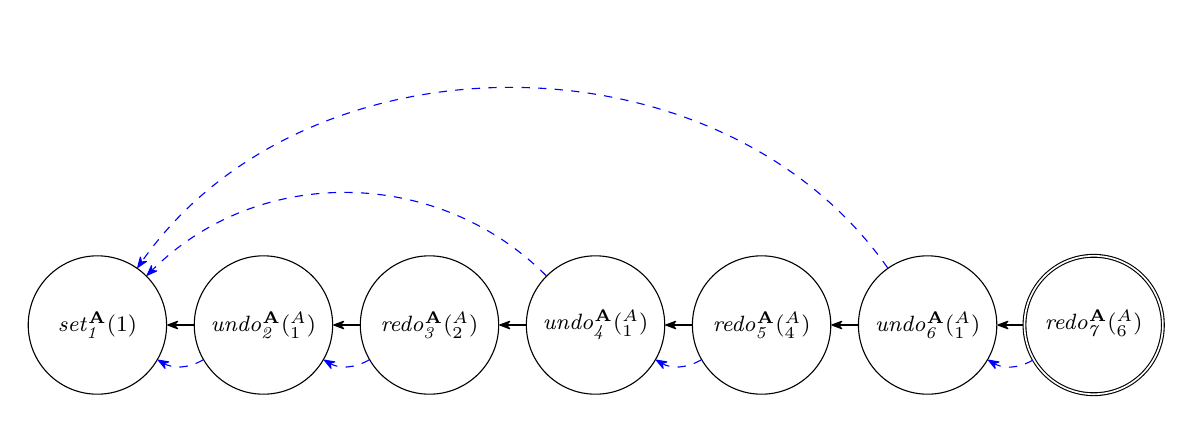
\begin{tikzpicture}[node distance=60pt]

        \node[op] (a1) at (0, 0) {\setop{1}{A}{1}};
        \pause
        \node[op,right of=a1] (a2) {\undop{2}{A}{1}{A}} edge [pred] (a1) edge [anchorref,bend left] (a1);
        \node[op,right of=a2] (a3) {\redop{3}{A}{2}{A}} edge [pred] (a2) edge [anchorref,bend left] (a2);
        \pause
        \node[op,right of=a3] (a4) {\undop{4}{A}{1}{A}} edge [pred] (a3) edge [anchorref,bend right=45] (a1);
        \node[op,right of=a4] (a5) {\redop{5}{A}{4}{A}} edge [pred] (a4) edge [anchorref,bend left] (a4);
        \pause
        \node[op,right of=a5] (a6) {\undop{6}{A}{1}{A}} edge [pred] (a5) edge [anchorref,bend right=55] (a1);
        \node[head,right of=a6] (a7) {\redop{7}{A}{6}{A}} edge [pred] (a6) edge [anchorref,bend left] (a6);

      \end{tikzpicture}
    \end{adjustbox}
    \caption{Sequence of alternating undo-redo operations\only<1>{.}
    \only<2->{of length }\only<2>{1}\only<3>{2}\only<4>{3}\only<2->{.}
    }\label{fig:degenerate-editing-scenario}
  \end{figure}
\end{frame}

\begin{frame}{Linear Runtime for Impractical Scenarios}
  \begin{figure}
    \begin{adjustbox}{max totalsize={\textwidth}{0.75\textheight},center}
      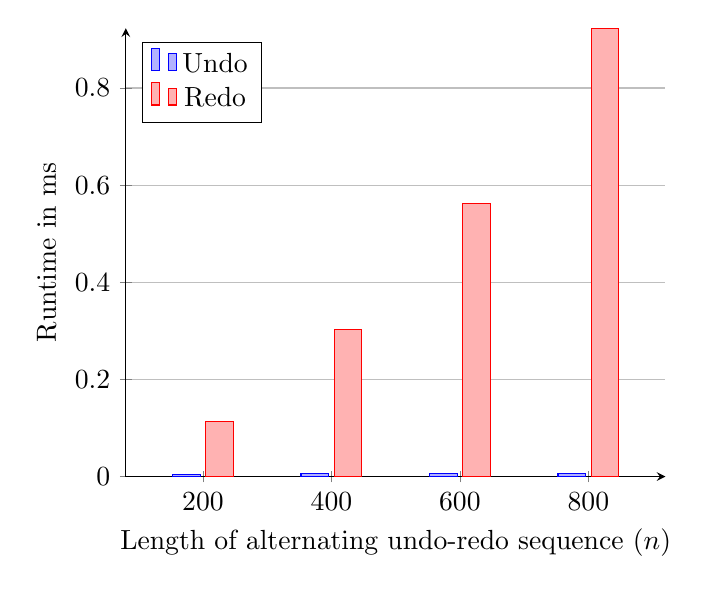
\begin{tikzpicture}
      \begin{axis}[
        ybar,
        ylabel={Runtime in ms},
        axis y line=left,
        ymin = 0,
        xlabel={Length of alternating undo-redo sequence ($n$)},
        axis x line=bottom,
        symbolic x coords={200, 400, 600, 800},
        ymajorgrids=true,
        yminorgrids=true,
        enlarge x limits = 0.2,
        legend pos = north west,
      ] 

      % undo
      \addplot+ coordinates {
      (200, 0.00504857866326347)
      (400, 0.005509669485036284)
      (600, 0.006512108666356653)
      (800, 0.007120864116586745)
      };

      % redo
      \addplot+ coordinates {
      (200, 0.11390662190387957)
      (400, 0.3034253417572472)
      (600, 0.5630059454997536)
      (800, 0.9230491668859031)
      }; 

      \legend{Undo, Redo};
      \end{axis} 
      \end{tikzpicture} 
    \end{adjustbox}
    \caption{
    Runtime of the last undo/redo operation
    in a sequence of alternating undo-redo operations of length $n$.
    }\label{fig:runtime-undo-redo-alt}
  \end{figure}
\end{frame}

\subsection{Undo Taxonomy}

\begin{frame}{A Taxonomy of Undo Behavior}
  \begin{table}
    \centering
    \begin{tabular}{@{}ccc@{}}
            Order $\backslash$ Origin
            & \makecell{Generating\\Replica}
            & \makecell{Any\\Replica}
            \\
        \midrule
            \makecell{Reverse\\ Chronological}
            & \alert{local undo}
            & global undo
            \\
        \midrule
            Selective
            & \multicolumn{2}{c}{revert\footnote{often called \emph{selective undo} in the literature~\cite{Yu2015undo}}}
            \\
    \end{tabular}
  \end{table}
\end{frame}

\begin{frame}[fragile]{Undo Kinds in a Collaborative Setting}
  \begin{figure}
    \center
    \begin{adjustbox}{max totalsize={\textwidth}{0.75\textheight},center}
        \tikzset{
          treenode/.style = {shape=rectangle, rounded corners,
                             draw, align=center,},
          root/.style     = {treenode},
          dummy/.style    = {circle,draw}
        }
        \begin{tikzpicture}
          [
            grow                    = right,
            sibling distance        = 6em,
            level distance          = 10em,
            edge from parent/.style = {draw, -latex},
            every node/.style       = {font=\footnotesize},
            sloped
          ]
          \node [root,dummy] {}
            child { node [treenode, align=center] {selective undo}
              edge from parent node [below] {any order} }
            child { node [treenode] {undo}
              child { node [treenode] {global undo}
                edge from parent node [below] {all ops} }
              child { node [treenode] {local undo}
                edge from parent node [above, align=center] {own ops} }
              edge from parent node [above, align=center] {rev. chron. order} };
        \end{tikzpicture}
      \end{adjustbox}
  \end{figure}
\end{frame}

\end{document}
